\chapter{Generation}\label{ch:generation}

% ---------------------------------------------------------------------------
% RQ2. Same five-part shape as Chapter 5 (manifest §4a). Generation has no separate
% guards section: its one guard -- that every condition receives the same prompt --
% is a single argument and lives inside §6.2 where the prompt is presented.
%
% BLOCKED on the generation re-run -- manifest §15 O-1. Every number currently
% available was produced under the retired prompt asymmetry. ONE prompt is now
% presented, called "the answer-generation prompt", with NO version number; the
% files keep v3 and the artefact ledger (manifest §13) carries the mapping.
% Never write: coverage, selective, composite, refusal. Each measure is one number.
% ---------------------------------------------------------------------------

% Chapter 6 section 6.1: overview.
% Written 2026-09-26 (manifest §9b row 6.1), drafted in the chat and approved before this write.
% Shape follows §5.1 as rewritten 2026-09-25: no verbatim RQ block and no mapping table (§15 O-20 c),
%   no float, no ranking clause (review E4), ~250 words.
% Carries: the road map; the recap of which configuration "the multi-index retriever" names -- the
%   blocked system, as §5.6 selects it, with no numbers repeated; FC-P introduced for the chapter;
%   faithfulness stated once as attribution rather than quality (manifest §1c); and the reading rule --
%   generation differences read as reported, §5.1's 0.02 belonging to retrieval scores alone.
% Not here: the RQ text, k, the generator sizes and the prompt (all §6.2); any oracle condition
%   (not reported -- manifest §9b, 2026-09-26).
% RQ3 is named as a sanity check on RQ2, her own term for it (susanne-review-response.md F8).
% The verdicts section is described rather than \ref'd: §6.4 has no label until it is written.

\section{Overview}\label{sec:gen-overview}

This chapter answers the second research question, on generation, and the third, a sanity
check on the second: whether its answers survive a change of generator.
Section~\ref{sec:gen-method} states how the answers were produced and how they were
scored. Section~\ref{sec:gen-results} reports three experiments: how answers generated
from the multi-index retriever's context compare with answers generated from no context and
from the context of text-only retrieval; whether answer quality tracks retrieval quality
across the fifteen retrieval configurations of
Section~\ref{sec:met-retrieval-configs}; and whether both results hold as the generator
grows. The chapter closes by ruling on each hypothesis.

The retriever this chapter gives the generator is the one Section~\ref{sec:ret-verdicts}
selected, the blocked multi-index system, and the retrieval it is set against is the
strongest text-only system, dense retrieval on its own. Both were chosen there by reading the
retrieval results, and this chapter takes them as given.

Two measures are reported, and they answer different questions. Factual-correctness precision
(FC-P) is the quality measure: the share of an answer's claims that the reference supports.
Faithfulness measures attribution rather than quality --- the share of an answer's claims that
the retrieved context supplied --- so a low value on a \emph{correct} answer means the
generator already knew the answer, not that the answer is poor. Faithfulness needs a context
to be computed against, and generation without retrieval therefore has no value for it.

Retrieval quality enters as the primary measure of Chapter~\ref{ch:retrieval},
nDCG$'$@10 under the labels of the relevance judge of
Section~\ref{sec:met-judge-validation}. Differences between generation scores are read as the
values are reported, with no statistical test and no equivalent limit: the 0.02 of
Section~\ref{sec:ret-overview} is a property of the relevance judge and governs retrieval
scores alone.


% Chapter 6 section 6.2: method.
% Rewritten 2026-09-26 (manifest §9b row 6.2), drafted in the chat and approved before this write.
% Replaces the version of 2026-09-15, which described the retired two-template design (v1/v2),
%   3B as the primary generator, the refusal string, 1024 tokens and the context-depth sweep.
% Carries: what was generated (floor defined at first use; the fifteen configurations of §5.2.2; the
%   two larger generators for RQ3); the context size as a design choice; ONE prompt, as Figure 6.1,
%   with no version number anywhere (CLAUDE.md §5); the generator settings as Table 6.1; reference
%   construction, with the community-score ordering §4.1 points here for; the two measures as RAGAS
%   computes them; faithfulness's missing upper anchor; and how the association is reported.
% Deliberately NOT here: faithfulness as attribution (stated once in §6.1); any oracle condition
%   (not reported -- manifest §9b, 2026-09-26); FC-recall (not reported -- same note); the word
%   "condition" (optional per §7a, and dropped); any depth sweep.
% Numbers to register in R9 before this is quoted elsewhere: no answer reached the token ceiling;
%   74 of 78 topics take a full five-answer reference; one faithfulness score is undefined (3B text
%   fusion); claim counts mean 6, median 6, range 1-22 over the 2,118 of 2,184 reported answers whose
%   score file records n_claims (the 3B blocked run does not record it for 63 of its 78 answers).
% Model revisions are NOT pinned (configs/task_c/generation_eval.yaml says revision: main), so the
%   section claims no pinning; the template itself lives in the run records, not in prompt_template.py.
% Floats: both captions sit below their content (review E3). Check placement on the build -- one
%   table that cannot be placed defers every later table in the chapter (§15 float-discipline note).
%   Width (fixed 2026-09-26): the listing is hand-wrapped to 62 characters, just inside the 63 the
%   the widest line the frame holds at \footnotesize; Table 6.1's two sanity-check generators sit on
%   separate lines because both names in one cell ran the tabular 115pt past the text block.

\section{Method}\label{sec:gen-method}

Section~\ref{sec:bg-generation-metrics} defined retrieval-augmented generation and the two
measures this chapter reports, and Section~\ref{sec:met-system-overview} placed the generator at
the end of the pipeline: the highest-ranked answers of a ranking become its context, and one fixed
prompt turns the question and that context into an answer. This section states what was generated,
from which contexts, and how the answers were scored. There is no query rewriting, no reranking, no
agentic loop and no adjustment of the prompt from one set of answers to the next.

\subsection*{What was generated}

Three sets of answers, all on the 78 topics of Section~\ref{sec:met-collection}. The first receives
no context at all: the generator is given the question alone and answers from its own knowledge.
This is the \emph{floor}, the level any retrieved context has to improve on. The second set comes
from the fifteen retrieval configurations of Section~\ref{sec:met-retrieval-configs}, each supplying
the five highest-ranked answers of its own ranking as the context for that topic. The third repeats
part of that work at two larger generators, for the sanity check the third research question asks:
the floor and five of the fifteen configurations --- the two text indexes, their fusion, the formula
block and the blocked system --- are generated again at 3 and at 7 billion parameters. Everything
else is held fixed, so what separates any two sets of answers is the context the generator was
given, and in the third set the size of the generator as well.

A context of five answers is a design choice rather than a measured optimum. It matches the size of
the reference the answers are scored against, and it is held fixed everywhere, so that no comparison
mixes a difference in how much context was supplied with a difference in which retrieval supplied
it. No sweep over that size is run.

\subsection*{The prompt}

Figure~\ref{fig:gen-prompt} shows it, and one template serves everything in this chapter. It
presents the retrieved answers, asks for the question to be answered, and permits the generator its
own knowledge alongside the context while asking it to prefer the context where the two conflict. It
instructs no refusal, so a weak context still yields an answer rather than a decline. When there is
no context the retrieved-context block disappears and the rest of the template is unchanged, which
is how the floor is generated: the floor and every retrieval configuration render from the same
template. That is what makes Section~\ref{sec:gen-results} a comparison of contexts.

\begin{figure}[t]
\begin{lstlisting}[frame=single,numbers=none,basicstyle=\ttfamily\footnotesize,
  breaklines=false,columns=fullflexible,xleftmargin=1em]
[SYSTEM]
You are a mathematics question-answering assistant. Answer the
question as accurately and completely as you can, and write
all mathematics in LaTeX. Retrieved context may be provided
below; when it is, use it wherever it helps, and prefer it
over your own recollection where the two conflict. You may
also draw on your own knowledge, whether or not retrieved
context is provided. Give the reasoning needed to justify the
answer, without restating the question or padding.

[USER]
Retrieved context:
[1] <first retrieved answer>

[2] <second retrieved answer>

    ...

[5] <fifth retrieved answer>

Question:
<the topic's title and question body>

Answer:
\end{lstlisting}
\caption[The answer-generation prompt]{The answer-generation prompt. One template serves every set
of answers in this chapter. The retrieved answers are numbered in the order the ranking returns them
and stand here as placeholders. When no context is supplied the \emph{Retrieved context} block is
absent and the rest of the template is unchanged, which is how the answers without context --- the
floor --- are generated. The system message is a single line in the template and is wrapped here to
fit the page.}
\label{fig:gen-prompt}
\end{figure}

\subsection*{The generator}

Table~\ref{tab:gen-settings} lists the settings. Decoding is greedy: the temperature is zero, so the
generator always takes the most probable next token, and answers are produced one prompt at a time.
Each setting was generated once, and greedy decoding leaves nothing to average --- with the
temperature at zero and the seed fixed, a repeat of the same setting returns the same answers. The
limit on new tokens is 2{,}048, and no answer reached it, so every answer was scored whole rather
than broken off in mid-derivation.

\begin{table}[t]
\centering
\begin{tabular}{ll}
\toprule
Setting & Value \\
\midrule
Generator                & \texttt{Qwen/Qwen2.5-1.5B-Instruct} \\
Generators, sanity check & \texttt{Qwen/Qwen2.5-3B-Instruct} \\
                         & \texttt{Qwen/Qwen2.5-7B-Instruct} \\
Precision                & bfloat16 \\
Temperature              & 0.0 \\
Top-$p$                  & 1.0 \\
Maximum new tokens       & 2{,}048 \\
Seed                     & 42 \\
Runs per setting         & 1 \\
Context size             & 5 answers \\
\addlinespace
Scoring framework        & RAGAS 0.4.3 \\
Scoring model            & \texttt{gemini-3.5-flash-lite}, temperature 0 \\
Claim decomposition      & atomicity high, coverage high \\
\bottomrule
\end{tabular}
\caption[Generation and scoring settings]{Generation and scoring settings. Every answer in this
chapter is produced and scored with these settings; the generator changes only where its size is the
thing being varied. \emph{Atomicity} and \emph{coverage} govern how finely a text is decomposed into
claims (Section~\ref{sec:bg-generation-metrics}). The scoring model is the one the scoring framework
uses for its own judgements, and is not the relevance judge of
Section~\ref{sec:met-judge-validation}.}
\label{tab:gen-settings}
\end{table}

\subsection*{The reference}

Factual correctness needs a reference, and Section~\ref{sec:bg-generation-metrics} left what it is
built from to this section. It is built from the assessors' judgments alone, never from the relevance
judge's labels, which would otherwise grade the pipeline against labels its own judge supplied. A
mathematics question usually admits several valid routes to the same result, so a single answer taken
as the reference would mark a correct answer wrong for having taken another route. The reference is
therefore the union of up to five judged answers for the topic: High-labelled answers first, filled
from Medium where a topic has fewer than five, and ordered within a label by the community score the
collection records. Seventy-four of the 78 topics have five or more such answers and take the full
five; the remaining four take the two, three or four they have. No topic is scored without a
reference.

\subsection*{The measures as computed}

Both are computed with RAGAS 0.4.3, whose own language model performs every judgement. It is the
same model the relevance judge of Section~\ref{sec:met-judge-validation} uses, doing a different task
as a different instrument; nothing in that section validates it.

Faithfulness is computed in two steps. The model first rewrites the answer into standalone
statements, each understandable without the others. It then judges each statement against the
retrieved context taken as one body of text and returns a verdict with a reason. The score is the
share of statements it can infer from the context. Where an answer yields no statements at all the
score is undefined rather than zero, which happens once across the runs reported here.

FC-P follows the same shape with the reference in place of the context. The model decomposes the
answer into claims and checks each against the reference; the reference itself is never decomposed,
so the score is the share of the answer's claims that the reference supports. Both parameters
Section~\ref{sec:bg-generation-metrics} names are set high --- atomicity, so that a sentence is split
into its indivisible claims, and coverage, so that the detail of each survives the split --- and the
setting is the same for every answer in this chapter. Across the answers reported here the
decomposition yields six claims on average, with a median of six and a range from one to twenty-two.
The framework rounds each factual-correctness score to two decimals. Faithfulness and FC-P decompose
the same answer separately, so the two scores are not fractions of one set of claims.

Read together, the two measures say where an answer came from. Because the generator is never
required to confine itself to the context, a correct answer may be its own work or the context's, and
the pair distinguishes the two: a high FC-P with a low faithfulness is a correct answer the generator
largely wrote from what it already knew, while a high FC-P with a high faithfulness is a correct
answer the context supplied. What the pair cannot supply is a ceiling for faithfulness. Since no
answer here was written under an instruction to use the context alone, faithfulness is read as a
share of what the answer says and never as a distance from an attainable maximum.

\subsection*{Relating answer quality to retrieval quality}

Two hypotheses read an association across configurations rather than a comparison between two sets of
answers. Retrieval quality is nDCG$'$@10 under the judge labels of
Section~\ref{sec:met-evaluation-protocol}, the primary measure of Chapter~\ref{ch:retrieval}, over
the same fifteen configurations. The association is reported as the Kendall's $\tau$ of
Section~\ref{sec:bg-agreement}, computed over all 105 pairs of those fifteen. It is computed on the
means before rounding, and it is reported for its sign and its size. No statistical test is applied
to it.

The sanity check reads the same coefficient over the five configurations generated at all three sizes
--- ten pairs --- and reads them at 1.5 billion parameters as well, so that the three sizes are
compared on one instrument. Those three values may be set beside one another; none of them may be set
beside the coefficient over fifteen configurations, which is computed from ten times as many pairs.


% Chapter 6 section 6.3: results -- 6.3.1 overview and 6.3.2, written 2026-09-26.
% Drafted in the chat and approved before this write (CLAUDE.md §2 steps 5-6).
% Structure fixed 2026-09-26 (Abram), manifest §9b row 6.3: an overview and THREE experiments.
%   6.3.1 overview
%   6.3.2 What the retrieved context changes        -> H2.1, H2.2   [written]
%   6.3.3 whether better retrieval reaches the answer -> H2.3, H2.4 [to come: one scatter,
%         two y axes, Kendall's tau on each, no p-value]
%   6.3.4 generator size, answering RQ3             -> H3.1         [to come: ten pairs, not
%         105, said once; cross-size ordering as an observation with no verdict]
% The oracle ceiling is NOT reported (manifest §9b, 2026-09-26). No depth sweep (2026-09-19).
% Every number here is manifest §14 R9 (registered 2026-09-26, O-23 closed). NO R8 figure.
% Headings name what is studied: no hypothesis ID and no verdict in a heading (CLAUDE.md §5).
% No numbered subheadings inside a subsection -- bold lead-ins (manifest §4b).
% No 0.02 limit in this chapter: it is the relevance judge's and governs retrieval scores
%   alone (§6.1). No test, no interval, no "significant" (manifest §1c-i).
% The verdicts are §6.4's. This section says which rule each hypothesis reads and stops.
% §6.4 landed 2026-09-26: the three placeholders are now \ref{sec:gen-verdicts}.
% Float: [!t] deliberately. Table 6.1 and Figure 6.1 are already queued in §6.2, and one table
%   that cannot be placed defers every later table in the chapter, silently (manifest §15).

% ⚠ WORDING REPAIRED 2026-09-27 (Abram), with the §7.1 write. SLT-TYPE's answers are "nonetheless
%   NOT DRAGGED BELOW the floor, at 0.196", not "nonetheless above the floor". A per-topic check of
%   the 1.5B per-sample score files (DIAGNOSTIC ONLY -- not registered, not reportable, not citable)
%   shows the 0.196-against-0.170 gap is five topics rescued from zero factual correctness, with a
%   median per-topic difference of 0.000, so "above the floor" states a five-topic tail as a level.
%   §6.4 carries the matching repair and §7.1 uses the same words. UNCHANGED deliberately: the
%   ten-above / five-below count earlier in this subsection and §6.3.3's "stands above eight of the
%   fourteen" -- both are counts over the reported means, not causal claims, and three sections
%   argue from them. Snapshot `_sec63_results.preFloorWording.bak.tex`.
\section{Results}\label{sec:gen-results}

\subsection{Overview}\label{sec:gen-res-intro}

Three experiments answer the questions this chapter asks, and they run in the order the
argument needs. The first two change what the generator is given and hold everything else
fixed: whether a retrieved context reaches the answer at all, and then whether a better
context reaches it further. The third changes the generator rather than the context,
repeating both at three and at seven billion parameters.

% --------------------------------------------------------------------------------------------
\subsection{What the retrieved context changes}\label{sec:gen-res-context}

A retrieval system that ranks better does not thereby produce a better answer. The generator
may ignore what it is given, or use it and be carried wrong by it, and nothing in
Chapter~\ref{ch:retrieval} says which happens. This section puts three settings beside one
another on the 1.5-billion-parameter generator: no context at all, the context of the
strongest text-only retrieval, and the context of the multi-index retriever. One template
serves all three, so what separates them is the context.

Two hypotheses read these answers. Hypothesis H2.1 predicts that the multi-index retriever's
context makes answers more factually correct than generation without retrieval, and holds only
if the blocked system is ahead of the floor on FC-P. Hypothesis H2.2 predicts that the same
context makes answers both more factually correct and more faithful than the strongest
text-only retrieval's, and holds only if the blocked system is ahead of dense retrieval on
both measures. Neither reads a threshold: the values are read as they are reported.

\textbf{Against no context.} The floor reaches 0.170 FC-P over the 78 topics of
Section~\ref{sec:met-collection} and the blocked system 0.206, ahead by 0.036
(Table~\ref{tab:gen-res-context}). It is ahead on 33 of the 78 topics, behind on 23 and level
on 22; the scoring framework rounds each factual-correctness score to two decimals, which is
why so many topics come out level. Section~\ref{sec:gen-verdicts} rules on H2.1.

The floor is not the bottom of the field, though. Ten of the fifteen configurations of
Section~\ref{sec:met-retrieval-configs} stand above it on FC-P and five below --- OPT, SLT,
the formula block, dense with SLT-TYPE, and dense with the three formula rankings each voting
separately. A retrieved context is therefore not an improvement in itself. Below some level of
retrieval quality the answers built from a context are worse than answers written from none.

The one configuration that breaks the pattern marks what drives it. SLT-TYPE alone is the
weakest retrieval of the fifteen and its answers are nonetheless not dragged below the floor,
at 0.196, while their faithfulness is the lowest in the chapter at 0.049 --- almost nothing they say
comes from the context (Figure~\ref{fig:gen-res-tau}). Each of the five that fall below the floor draws on its context more
than that. A context weak enough to be ignored costs the generator nothing, and a context used
but wrong costs it the answer.

\textbf{Against the strongest text-only retrieval.} Section~\ref{sec:ret-verdicts} found the
two systems indistinguishable as retrieval, 0.551 against dense retrieval's 0.557 on
nDCG$'$@10. Their answers are not indistinguishable. On faithfulness the blocked system is
ahead, 0.189 against 0.171, and ahead on 37 topics against 33; on FC-P it is behind, 0.206
against 0.241, and behind on 39 topics against 24. H2.2 needs both, so the correctness half
decides it, and Section~\ref{sec:gen-verdicts} rules on it.

The two measures answer different questions, as Section~\ref{sec:gen-overview} set out, and
here they answer in opposite directions. More of what the generator says under the multi-index
context is traceable to that context, and less of what it says is right. The multi-index
context is used more and helps less.

Two comparisons read two points each, and the field has fifteen. Whether where a context sits
in the retrieval ordering predicts anything about the answers built from it is the question
the next section asks of all fifteen at once.

\begin{table}[!t]
\centering
\small
\renewcommand{\arraystretch}{1.15}
\begin{tabular}{lrrr}
\toprule
Context & nDCG$'$@10 & Faithfulness & FC-P \\
\midrule
No context --- the floor & ---   & ---   & 0.170 \\
Dense retrieval          & 0.557 & 0.171 & \textbf{0.241} \\
Blocked multi-index      & 0.551 & \textbf{0.189} & 0.206 \\
\bottomrule
\end{tabular}
\caption[What the retrieved context changes]{Answers generated without a context, from dense retrieval's context, and from the
blocked multi-index retriever's. \emph{nDCG$'$@10}: prime normalised discounted cumulative
gain at rank 10, the retrieval quality of Chapter~\ref{ch:retrieval}. \emph{FC-P}:
factual-correctness precision. Faithfulness is undefined without a context. The 78 topics of
Section~\ref{sec:met-collection}, five retrieved answers as context, 1.5-billion-parameter
generator. The highest value in each of the two answer-quality columns is set in bold.}
\label{tab:gen-res-context}
\end{table}

% --------------------------------------------------------------------------------------------
% 6.3.3 written 2026-09-26, drafted in the chat over two passes and approved before this write.
% Vocabulary is §3.6's own: two ORDERINGS of the same systems, CONCORDANT and DISCORDANT pairs.
%   The word "association" is deliberately not used here (§6.2 still carries it twice -- sweep
%   together or leave, Abram's call, raised 2026-09-26).
% Numbers: manifest §14 R9.B, including the discordance breakdown registered the same day.
%   NO SUBSET TAU is computed or reported -- the rules read all 105 pairs and a coefficient over
%   a chosen subset would be a re-fit (CLAUDE.md §5).
% Cut on Abram's instruction, 2026-09-26: the closing caution paragraph (that the two values
%   describe the fifteen taken together and say nothing about a small gain at the top of the
%   range, with dense vs blocked as the case in point).
% Figure 6.2 added 2026-09-26 (Abram's choice, shown in the chat): TWO PANELS sharing the x axis,
%   not the two y axes manifest §9b specifies -- on one pair of axes the two clouds overlap and the
%   eye compares heights measured against different scales. Both series are round markers, the
%   chapter's two blues. Generated by experiments/diagnostics/plot_generation_tau_figure.py, which
%   recomputes both tau from the per-answer score files and reproduces R9's values exactly.
%   ONE \ref only, at the result sentence -- Abram's instruction, references only where needed.
% §6.4 landed 2026-09-26: the three placeholders are now \ref{sec:gen-verdicts}.

\subsection{Retrieval quality and answer quality}\label{sec:gen-res-tau}

% Float placement: declared HERE, immediately after the heading, not at the end of the
%   subsection. A [t] float can only reach the top of a page LATER than its declaration
%   point, so declared at the end of §6.3.3 -- which sat on page 73 -- it was deferred to
%   page 74. Declared at the head of §6.3.3, while the page is still 72, the first top it
%   can reach is page 73. [!t] waives the placement fractions for this float alone
%   (manifest §15 float-discipline note). Figures queue separately from tables, so Table 6.2
%   is unaffected. Re-check the page numbers in ausarbeitung.aux after the build, not by eye.
\begin{figure}[!t]
\centering
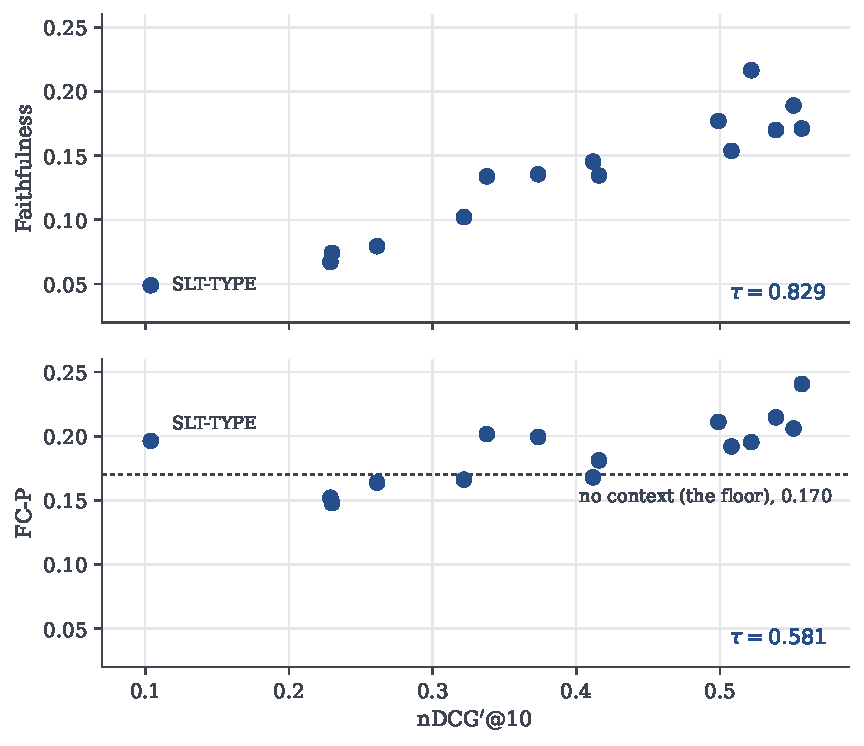
\includegraphics[width=0.82\textwidth]{images/gen_tau_retrieval_quality.pdf}
\caption[Answer quality against retrieval quality]{Faithfulness and factual-correctness precision (FC-P) of the generated answers, against
the retrieval quality of the configuration that supplied the context, over the fifteen
configurations of Section~\ref{sec:met-retrieval-configs}. Kendall's $\tau$ in each panel, over
all 105 pairs. The dashed line marks generation without retrieval, which has an FC-P but no
faithfulness and so appears in the lower panel alone. SLT-TYPE is named in both panels as the
configuration the surrounding text argues from. \emph{nDCG$'$@10}: prime normalised discounted
cumulative gain at rank 10, under the judge labels. The 78 topics of
Section~\ref{sec:met-collection}, five retrieved answers as context, 1.5-billion-parameter
generator.}
\label{fig:gen-res-tau}
\end{figure}

The two comparisons of Section~\ref{sec:gen-res-context} each read a pair of systems, and a pair
cannot say whether the relation holds in general: two systems may differ for reasons that have
nothing to do with how well either retrieved. The fifteen configurations can answer it, because
they retrieve at very different levels --- from 0.104 to 0.557 nDCG$'$@10.

Two hypotheses put the question, one for each measure. Hypothesis H2.3 predicts that faithfulness
rises with the quality of the retrieved context: the better the context, the more of the answer
comes from it. Hypothesis H2.4 predicts the same of factual correctness. Each is rejected if its
measure does not rise with retrieval quality across the fifteen. Every pair enters the Kendall's
$\tau$, and no resolving power is applied to it: the 0.02 of
Section~\ref{sec:met-judge-validation} sets no pair aside as too close to order.

Both measures rise with retrieval quality (Figure~\ref{fig:gen-res-tau}). Ordering the fifteen by retrieval quality and again by
faithfulness leaves the two orderings concordant on 96 of the 105 pairs, $\tau = 0.829$. Ordering
them by factual correctness instead leaves 83 of 105 concordant, $\tau = 0.581$. The closing
section of this chapter rules on H2.3 and H2.4.

Read together, the two say more than either does alone. The generator draws on the context it is
given, and the better that context, the more of the answer comes from it: only 9 of the 105 pairs
run the other way. Correctness rises too, and less evenly, with 22 pairs out of order. The chain
from retrieval to the answer has two links and they are not equally tight. A better context is
more likely to be used, and being used is not the same as being right.

Where correctness runs backwards is worth naming. Eight of its 22 discordant pairs involve
SLT-TYPE alone. It retrieves worst of the fifteen and its faithfulness is the lowest in the
chapter, 0.049, so the generator hardly touches what it supplies and writes much the same answer
it would write from no context at all. At 0.196 that answer stands above eight of the fourteen
configurations that retrieve better than it does (Figure~\ref{fig:gen-res-tau}). A context the generator does not use cannot pull
its answers down to the level of the retrieval behind it.

Both orderings are read on the smallest generator, on the same fifteen contexts throughout.
Whether either survives a larger one is the last question this chapter asks.

% --------------------------------------------------------------------------------------------
% 6.3.4 written 2026-09-26, drafted in the chat and approved before this write.
% Answers RQ3 and rules on nothing -- H3.1's verdict is §6.4's.
% Numbers: manifest §14 R9.C, including the below-floor counts registered the same day.
% Carries, as manifest §9b requires: RQ2.1's two comparisons repeated at each size; both measures
%   against retrieval quality over the five common conditions; the 1.5B value over those same five
%   as a REFERENCE POINT, not a test; the ten-pairs-against-105 caveat, stated once, as the reason
%   rather than the rule (§6.2 carries the comparability rule itself); and the cross-size ordering
%   as an OBSERVATION WITH NO VERDICT.
% ⚠ H3.1's CLAUSE (a) WAS RESTATED 2026-09-26 (Abram) and this section is written against the
%   restated wording: at 3B and 7B each of RQ2.1's three comparisons must run in the SAME DIRECTION
%   as at 1.5B. The rule drafted 2026-09-24 read absolute directions -- blocked ahead of dense on
%   BOTH measures -- which had operationalised the prior-form statement on the assumption that H2.2
%   would be supported; H2.2 was not, so that rule had become a restatement of H2.2's failed
%   condition and failed at all three sizes for a reason unrelated to generator size. Full note and
%   the disclosure in manifest §1c and §10 (the §7.2 post-hoc row).
%   THE VERDICT DOES NOT MOVE -- not supported either way: clause (b) fails at 3B on its own
%   (FC-P tau = 0.000) and clause (a) now fails at 7B. §6.4 must say that RQ2.1 REPLICATES AT 3B
%   and breaks at 7B, not that the experiment failed everywhere. This section states the directions
%   and rules on nothing.
% Float: Table 6.3 declared at the head of the subsection, not at its end -- a [!t] float can only
%   reach the top of a page LATER than its declaration point, which is what put Figure 6.2 a page
%   late. Tables queue in declaration order behind Tables 6.1 and 6.2; re-check every later table
%   in the chapter on the build, from ausarbeitung.aux (manifest §15 float-discipline note).

\subsection{The size of the generator}\label{sec:gen-res-sizes}

\begin{table}[!t]
\centering
\small
\setlength{\tabcolsep}{4.5pt}
\renewcommand{\arraystretch}{1.15}
\begin{tabular}{lrrrrrrr}
\toprule
& & \multicolumn{2}{c}{1.5B} & \multicolumn{2}{c}{3B} & \multicolumn{2}{c}{7B} \\
\cmidrule(lr){3-4}\cmidrule(lr){5-6}\cmidrule(lr){7-8}
Context & nDCG$'$@10 & Faith. & FC-P & Faith. & FC-P & Faith. & FC-P \\
\midrule
No context --- the floor & ---   & ---   & 0.170 & ---   & 0.201 & ---   & 0.246 \\
\addlinespace
formula block            & 0.261 & 0.079 & 0.164 & 0.072 & 0.214 & 0.086 & 0.229 \\
BM25                     & 0.338 & 0.134 & 0.202 & 0.150 & 0.214 & 0.162 & 0.243 \\
BM25 + dense             & 0.539 & 0.170 & 0.215 & 0.174 & 0.204 & \textbf{0.225} & 0.272 \\
blocked                  & 0.551 & \textbf{0.189} & 0.206 & \textbf{0.214} & 0.214 & 0.197 & \textbf{0.281} \\
dense                    & 0.557 & 0.171 & \textbf{0.241} & 0.189 & \textbf{0.313} & 0.221 & 0.277 \\
\bottomrule
\end{tabular}
\caption[The three generator sizes]{The floor and the five configurations generated at all three generator sizes, ordered by
retrieval quality. \emph{Faith.}: faithfulness, undefined without a context. \emph{FC-P}:
factual-correctness precision. \emph{nDCG$'$@10}: prime normalised discounted cumulative gain at
rank 10, under the judge labels. \emph{1.5B}, \emph{3B}, \emph{7B}: generators of 1.5, 3 and 7
billion parameters. The 78 topics of Section~\ref{sec:met-collection}, five retrieved answers as
context. The highest value in each faithfulness and FC-P column is set in bold; the nDCG$'$@10
column orders the rows and is not marked.}
\label{tab:gen-res-sizes}
\end{table}

Everything so far is read on a 1.5-billion-parameter generator, the smallest of the three. A model
that size has less of its own to bring, so a retrieved context has more room to matter to it, and a
larger model may need it less. The third research question asks whether the answers to the second
survive that change. It is a sanity check on those answers rather than a question about generators
in their own right.

The floor and five of the fifteen configurations --- the two text indexes, their fusion, the formula
block and the blocked system --- were generated again at 3 and at 7 billion parameters, with the
prompt, the context size, the decoding and the topics all held fixed
(Table~\ref{tab:gen-res-sizes}). Hypothesis H3.1 predicts that the conclusions of the second
research question are not specific to the smallest generator, in two clauses. The first asks that
each of the three comparisons of Section~\ref{sec:gen-res-context} --- the blocked system against
the floor on FC-P, and against dense retrieval on FC-P and on faithfulness --- runs in the same
direction at the larger sizes as it does at the smallest. The second asks that both measures still
rise with retrieval quality there.

\textbf{The three comparisons at each size.} All three keep their direction at 3 billion
parameters; two of them reverse at 7 billion. Against the floor, the blocked system stays ahead on
FC-P throughout: 0.206 against 0.170 at 1.5 billion parameters, 0.214 against 0.201 at 3 billion
and 0.281 against 0.246 at 7 billion. That is the direction
Section~\ref{sec:gen-res-context} found, and both larger generators keep it. Against dense
retrieval the blocked system is behind on FC-P at the two smaller sizes, 0.206 against 0.241 and
0.214 against 0.313, and ahead at the largest, 0.281 against 0.277; on faithfulness it runs the
other way, ahead at the two smaller sizes, 0.189 against 0.171 and 0.214 against 0.189, and behind
at the largest, 0.197 against 0.221. Both of these match
Section~\ref{sec:gen-res-context} at 3 billion parameters and reverse at 7 billion. The two
reversals run in opposite senses: under the largest generator the blocked system's context produces
the more factually correct answers of the two, and supplies less of what those answers say.

\textbf{Retrieval quality at each size.} Over the five conditions common to all three sizes,
faithfulness rises with retrieval quality at every size: $\tau = 0.800$ at 1.5 billion parameters,
0.800 at 3 billion and 0.600 at 7 billion. Factual correctness rises at the smallest and the
largest, $\tau = 0.800$ in both, and at 3 billion it does not, $\tau = 0.000$, with five of the ten
pairs in one order and five in the other. The value at 1.5 billion is a reference point rather than
a test --- the clause reads the two larger sizes, and computing the same $\tau$ over the same
five conditions puts all three sizes on one instrument. All three are read over ten pairs where
Section~\ref{sec:gen-res-tau} reads 105, so a single pair changing places moves one of them by
0.200; they may be set beside each other and beside nothing else. Section~\ref{sec:gen-verdicts} rules on H3.1.

\textbf{What the ladder shows about generators.} One thing more is worth recording, and it
decides nothing. The floor's FC-P rises at every step in generator size: 0.170 at 1.5 billion
parameters, 0.201 at 3 billion and 0.246 at 7 billion. At 1.5 billion it stands above one of the
five conditions, at 3 billion above none, and at 7 billion above two --- BM25 at 0.243 and the
formula block at 0.229, against its own 0.246. Answers built from those two contexts are less
factually correct than answers built from no context at all. The larger the generator, the more of
the answer it already holds, and the better a retrieved context has to be before it adds anything.

% 6.3.1 and 6.3.2 written 2026-09-26. Still to come, in _sec63_results.tex:
%   6.3.3 whether better retrieval reaches the answer -> H2.3, H2.4. ONE scatter over the
%         fifteen configurations, two y axes, KENDALL'S TAU on each (never Spearman's rho --
%         manifest §1c), no p-value, no pair set aside under the 0.02 rule.
%   6.3.4 generator size, answering RQ3 -> H3.1. RQ2.1's two comparisons repeated at 1.5B /
%         3B / 7B, and both measures against retrieval quality over the five conditions common
%         to all three sizes -- ten pairs, not 105, and say so once. Cross-size ordering is an
%         observation with no verdict.
%   The oracle ceiling is NOT reported (manifest §9b, 2026-09-26) -- no ceiling subsection.
%   Context depth is DROPPED (2026-09-19) -- no k-sweep, no section.
% Old draft retained for reference only, NOT input: _sec63_results.BLOCKED.tex

% Chapter 6 section 6.4: the verdicts. Written 2026-09-26, drafted in the chat over three passes
%   and approved before this write (CLAUDE.md §2 steps 5-6).
% Shape mirrors §5.6 (manifest §9b): bold lead-ins, ~one page, no float, SUPPORTED / NOT SUPPORTED
%   only -- the three-point scale was dropped 2026-09-25 and "partially supported" is not used.
% Rules on H2.1, H2.2, H2.3, H2.4 and H3.1 against the decision rules of §1c, and answers RQ2.1,
%   RQ2.2, RQ3 and RQ2. Numbers are kept to what anchors a verdict: Abram's instruction was that
%   this section carry the argument as a story, not as a second pass over §6.3's tables.
% H3.1 is read against its clause (a) AS RESTATED 2026-09-26 -- each of RQ2.1's three comparisons
%   keeping its direction (manifest §1c). The verdict is the same under either wording; the wording
%   matters only so that "not supported" does not read as a blanket failure. RQ2.1 replicates at 3B.
% ⚠ H3.1's ORIGIN DISCLOSURE IS NOT HERE. Abram's instruction, 2026-09-26: the sentences naming the
%   superseded runs come out. H3.1 was stated before its own data, so nothing post-hoc happened to
%   the hypothesis itself; what IS owed is the clause (a) restatement, and that goes to §7.2 with
%   H1.3's. Manifest §9b row 6.4 and §10's post-hoc row are repointed to §7.2 accordingly. If §7.2
%   is written without it, the thesis discloses neither -- check when §7.2 lands.
% ⚠ ONE SENTENCE KEPT ON ABRAM'S EXPLICIT INSTRUCTION, against a reservation I raised in the chat
%   (2026-09-26): "How much of a context gets used follows from how pertinent it looks, which is
%   close to what a retrieval score measures." nDCG'@10 is computed under the judge labels, and
%   answer retrieval is graded on whether a post RESOLVES the question (§3.1, and §5.6 says so), so
%   "how pertinent it looks" is not a description of what the score measures. Four alternatives were
%   offered and this wording was chosen. Revisit if an examiner or the supervisor stops on it.
% Not here: the attenuation arc C-7 -- a retrieval difference reliable at the retrieval stage not
%   surviving into generation -- which needs both RQs and is §7.1's (manifest §10). Nothing from the
%   retired ladder. No third grade. No float.

% ⚠ WORDING REPAIRED 2026-09-27 (Abram), with the §7.1 write. Two changes in the first lead-in.
%   (i) "they land above the floor because the generator has effectively fallen back on its own
%   knowledge" -> "they are not dragged below the floor with it": the causal clause explained a
%   five-topic tail as though it were a level (see `_sec63_results.tex`'s note), and the two short
%   sentences after it already carry the mechanism, so the paragraph was explaining itself twice.
%   (ii) "A context it uses and that does not hold the answer costs it the answer." -> "A context it
%   draws on costs it the answer when the answer is not there." -- Abram's choice from three options;
%   the old sentence stacked two relatives on one omitted pronoun. §7.1 uses the same "not dragged
%   below" wording. Snapshot `_sec64_rq2_verdicts.preFloorWording.bak.tex`.
\section{What this settles about RQ2 and RQ3}\label{sec:gen-verdicts}

Section~\ref{sec:gen-results} ran three experiments, and each of them decides a hypothesis. A
retrieved context does reach the answer, and it reaches it in proportion to how good the retrieval
was. What it reaches is how much of the answer the generator borrows, and borrowing more is not the
same as being right more often.

\textbf{Whether a retrieved context helps at all.} H2.1 predicted that the multi-index retriever's
context makes answers more factually correct than generation without retrieval. It does: 0.206 FC-P
against the floor's 0.170 over the 78 topics of Section~\ref{sec:met-collection}, ahead on 33 of
them and behind on 23. H2.1 is supported. The result does not generalise to retrieval as such,
though. Five of the fifteen configurations fall below the floor, and the configuration that escapes
that pattern explains it: SLT-TYPE retrieves worst of all fifteen, its answers draw less on their
context than any other, and they are not dragged below the floor with it
(Figure~\ref{fig:gen-res-tau}). A context the generator ignores costs it nothing. A context it draws
on costs it the answer when the answer is not there.

\textbf{The multi-index retriever against text-only retrieval.} H2.2 predicted that its context
makes answers both more factually correct and more faithful than the strongest text-only
retrieval's. Only the second holds: 0.189 faithfulness against dense retrieval's 0.171, and 0.206
FC-P against 0.241. H2.2 is not supported, and the answer to RQ2.1 is yes to its first half and no
to its second. The two measures moving in opposite directions is the finding, and Chapter~5 has
already named its cause. The formula rankings put posts in front of the generator that share the
question's formulas, and Section~\ref{sec:res-transfer} established that formula containment
identifies the right neighbourhood and cannot order inside it. The generator does what the ranking
did: it treats those posts as pertinent and draws on them. Formula similarity attracts the
generator's attention without carrying the answer.

\textbf{Whether better retrieval reaches the answer.} H2.3 and H2.4 predicted that faithfulness and
factual correctness rise with retrieval quality across the fifteen configurations. Both do, and
both are supported, so the answer to RQ2.2 is yes. They do not rise equally: the ordering by
retrieval quality and the ordering by faithfulness agree on 96 of the 105 pairs, $\tau = 0.829$,
and by factual correctness on 83, $\tau = 0.581$. The chain from a retrieval score to a correct
answer has two links and only the first is tight. How much of a context gets used follows from how
pertinent it looks, which is close to what a retrieval score measures. Whether the answer comes out
right depends on whether that context actually held the answer, which a retrieval score measures
much less well.

\textbf{Whether any of it survives a larger generator.} H3.1 predicted that the answers to RQ2 are
not specific to the smallest generator. They are not robust to it. Every comparison holds its
direction at 3 billion parameters and two of the three reverse at 7 billion, and factual
correctness stops rising with retrieval quality at 3 billion altogether. H3.1 is not supported and
the answer to RQ3 is no --- though what fails is narrower than that verdict sounds, since RQ2.1
replicates cleanly at the middle size. The reason is visible in the floor: a generator that already
holds more of the answer raises the bar a context has to clear, and at 7 billion parameters two of
the five contexts fall below it.

\textbf{RQ2 and RQ3 as a whole.} One fact sits underneath all of it. The highest faithfulness
anywhere in this chapter is 0.225: in every configuration, at every generator size, most of what an
answer says comes from the generator rather than from what was retrieved. Retrieval is a minority
contributor to the text, and the rest follows from that. It is why the multi-index retriever's
context can be drawn on more heavily and still produce less correct answers. It is why a clean
ordering at the retrieval end arrives at the answer as a loose one. And it is why the whole effect
thins as the generator grows and has more of its own to offer. Retrieval reaches the answer; it
does not write much of it.

Chapter~\ref{ch:discussion} takes up what the two chapters say together, and what this thesis could
not measure.

